\subsection{Controlador de interruptores y atenuadores 11713 (Attenuator Switch Driver)}
Los equipos de la serie 11713 están diseñados para generar las señales de control o conmutación para bancos de atenuadores o interruptores electromecánicos para RF y \textmu, de acuerdo a la selección hecha por el usuario en su panel frontal o en forma de comando enviado de forma remota a este dispositivo a través de un bus GPIB, USB o una red LAN.
Los atenuadores e interruptores coaxiales electromecánicos que no dispongan de interfaz de usuario, se debe emplear un equipo de la serie 11713 para que el usuario pueda controlar a estos dispositivos.

El 11713 permite al usuario controlar un banco de interruptores o atenuadores interactuando con su interfaz física en su panel frontal (modo local) y también permite control en modo remoto, el usuario puede enviar comandos a través de un bus GPIB (modelo 11713A), un bus USB o una red LAN (modelos 111713B y 11713C).

Fabricado inicialmente por Agilent Technologies con el modelo 11713A (figura \ref{Fig:Versiones11713}a) actualmente es producido por Keysight Technologies, en dos versiones mejoradas pero que conservan toda la funcionalidad del equipo original de Agilent, en los equipos 11713B (figura \ref{Fig:Versiones11713}b) y 11713C (figura \ref{Fig:Versiones11713}c).

\begin{figure}[h!]
{
	\centering
	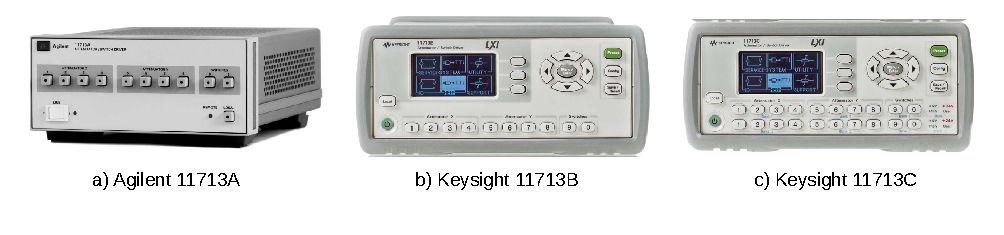
\includegraphics[width=\textwidth]{./Imagenes/Versiones11713.pdf}
	\caption{Versiones para los equipos de la serie 11713.}
	\label{Fig:Versiones11713}
}
\end{figure}

Los equipos de la serie 11713 pueden controlar una amplia gama de modelos de atenuadores o interruptores, en la tabla \ref{Tab:ModelosInterruptoresAgilent} se muestran los modelos compatibles de Agilent. Los interruptores a controlar pueden ser de tipo
SPDT, bypass, matrix, transfer y multipuerto.


\begin{table}[h!]
	\centering
	\begin{tabularx}{\textwidth}{cX}
		\toprule
		Tipo de interruptor	&	Modelos \\
		\midrule
		SPDT 				&	8761B, 8762A/B/C/F, 8765A/B/C/D/F, N1810TL, N1810UL \\
		\midrule 
		Bypass				&	8763A/B/C, 8764A/B/C, N1811TL, N1812UL \\
		\midrule			
		Multipuerto			&	87104A/B/C, 87204A/B/C, 87106A/B/C, 87206A/B/C, 8766K, 8767K, 8768K, 8769K, 8767M, 8768M, 8769M \\
		\midrule
		Matrix				&	87406B, 87606B \\
		\midrule
		Transfer			& 	87222C/D/E \\
		\bottomrule
	\end{tabularx}
	\caption{Modelos de interruptores Agilent/Keysight compatibles con el 11713}
	\label{Tab:ModelosInterruptores11713}
\end{table}

\begin{table}[h!]
	\centering
	\begin{tabular}{cc}
		\toprule
		Modelo de atenuador	 	&	Atenuación 			\\		
		\midrule
		8494G,H (33320G,H)		&	11 dB, paso 1 dB	\\
		\midrule
		8495G,H,K (33321 G,H,K)	&	70 dB, paso 10 dB 	 \\
		\midrule
		8496G,H (33322G,H)		&	110 dB, paso 10 dB   \\
		\midrule		
		8497K ( 33323K)			&	90 dB, paso 10 dB 	 \\
		\midrule		
		84904K,L (33324K,L)		&	11 dB, paso 1 dB 	\\
		\midrule		
		84906K,L ( 33326K,L)	& 	90 dB, paso 10 dB 	\\
		\midrule		
		84907K,L (33327K,L) 	& 	70 dB, paso 10 dB 	\\
		\bottomrule		
	\end{tabular}
	\caption{Modelos de atenuador Agilent/Keysight compatibles con el 11713}
	\label{Tab:ModelosAtenuadores11713}
\end{table}
Los equipos de la serie pueden manejar un numero de atenuadores o interruptores, según el modelos. En general, el modelo 11713C puede el doble de atenuadores e interruptores que el modelo 11713B.

Los equipos de la serie 11713 disponen de dos tipos de interfaces, una interfaz de usuario y una interfaz eléctrica. Los equipos 11713B y 11713C agregan una tercera interfaz de comunicaciones. Estos equipos no presentan una interfaz para señales de RF o UW, no manejan ni realizan mediciones sobre este tipo de señales.

La interfaz de usuario se encuentra en el panel frontal de estos equipos, en el 11713A consiste básicamente en tres grupos de pulsadores. Los equipos 11713B y el 11713C también disponen de pulsadores en su panel frontal y además agregan una pantalla LCD a la interfaz de usuario.

\begin{table}[h!]
	\begin{tabularx}{\textwidth}{cXXXX}
		\toprule
			&	&	11713A	&	11713B	&	11713C \\
		\midrule
		\multirow{5}{*}{Botones} & Control de \newline atenuadores X & 1 panel de 4 botones & 1 panel de 4 botones & 2 paneles de 4 c/u. \\
			&	Control de \newline atenuadores Y & 1 panel de 4 botones & 1 panel de 4 botones & 2 paneles de 4 c/u. \\
			& 	Control de \newline interruptores & 1 panel de 2 botones &  1 panel de 2 botones & 2 paneles de 2 botones c/u. \\
			& 	Teclas de flecha 	&	No	& Si	& Si \\
			& 	Preset, Config, Save/Recall	& No	&	Si	& Si \\
		\midrule
		Pantalla LCD	& No	& Si	& Si
	\end{tabularx}
	\caption{Características de interfaz de usuario en los equipos 11713}
	\label{Tab:CaracteristicasInterfazUsuario11713}
\end{table}


El 11713 presenta una interfaz eléctrica la cual entrega señales de control que permiten seleccionar un nivel de atenuación en los atenuadores o abrir y cerrar un interruptor coaxial. Esta interfaz es accesible por medio del panel trasero de los equipos de la serie 11713, en forma de conectores como se aprecia en la figura 8 un detalle del panel posterior del 11713B. En este panel se encuentran los conectores con las señales de control para atenuadores e interruptores coaxiales. 

\begin{table}[h!]
	\begin{tabularx}{\textwidth}{XXXX}
		\toprule
				& 11713A	& 	11713B	&	11713C \\
		\midrule
		Control de atenuadores (pares de conector Viking de 12 pines)	& 1 par & 1 par & 2 pares \\
		\midrule
		Control de interruptores coaxiales (pares de jacks banana)	& 1 par (A y B) & 1 par (A y B) & 2 pares (A y B) \\
		\midrule
		Alimentación DC en los puertos & +24 V DC & +24 V DC +5, +15, +24 V DC, ajustable por usuario \\
		\midrule
		Control TTL & No & No & Si \\
		\midrule
		Cantidad máxima de atenuadores & 2 de 4 secciones & 2 de 4 secciones & 4 \\
		\midrule 
		Cantidad máxima de interruptores & 2 en los jacks banana. Hasta 10 SPDT en los conectores Viking & 4 en los jacks banana. Hasta 10 SPDT en los conectores Viking & 2 en los jacks banana. Hasta 20 SPDT en los conectores Viking. \\
		\bottomrule
	\end{tabularx}
	\caption{Interfaz eléctrica en los equipos 11713}
	\label{Tab:Interfaz eléctrica en los equipos 11713}
\end{table}

En un banco de atenuadores, como los de Agilent, la cantidad de atenuación que se introduce en el camino de señal es determinada por apertura o cierre de un un conjunto de interruptores electromecánicos, que insertan o retiran atenuadores en el camino de señal. Los interruptores coaxiales también emplean interruptores electromecánicos. Las
señales de comando que el 11713 envía a los interruptores electromecánicos es una señal de potencia, de tipo lógico y referidas a tierra.

Las señales de control para los modelos de atenuadores Agilent se encuentran en los conectores Viking. Existe un par de éstos en los modelos 11713 A y B, etiquetados como ATTEN X y ATTEN Y. El modelo 11713C dispone de dos pares de conectores Viking. Las señales presentes en los conectores Viking también pueden emplearse para el control de interruptores electromecánicos coaxiales.

La conexión entre un equipo de la serie 11713 con un atenuador o un interruptor coaxial se realiza por medio de cables especiales que se insertan en los conectores que disponen estos equipos. La información sobre modelos de cable de acuerdo al modelo de atenuador o interruptor se ofrece en las hojas de datos en forma de matrices de selección. Los
cables de conexión se eligen de acuerdo al numero de opción de los equipos 11713 y de acuerdo al modelo del equipo atenuador o interruptor, ubicando estos datos en la matriz de selección. La matriz de selección remite a una figura en donde se indica un esquema con instrucciones para realizar las conexiones entre éstos equipos. 

\begin{figure}[h!]
	\centering
	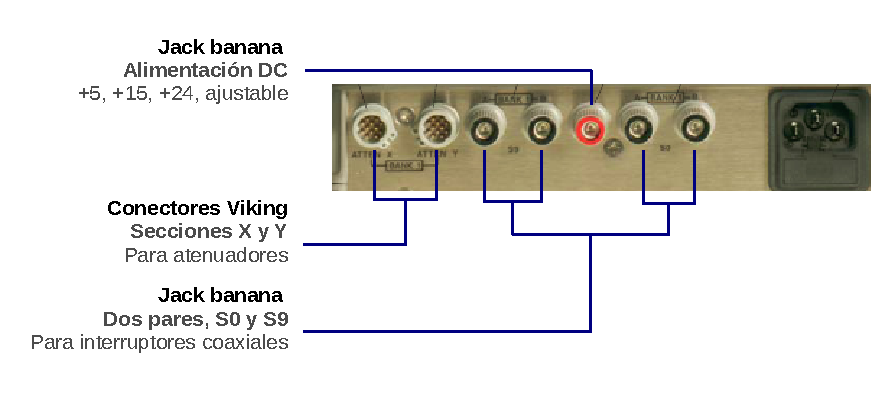
\includegraphics[width=0.8\textwidth]{Imagenes/SeccionPanelPosterior11713.pdf}
	\caption{Sección del panel posterior del 11713B}
	\label{Fig:SeccionPanelPosterior11713}
\end{figure}

Existe un modelo de cable apropiado para cada modelo de atenuador o interruptor coaxial, pero uno de sus extremos siempre debe poseer un conector Viking hembra si se desean utilizar éstos con un equipo 11713. 

\ Un conector Viking en el equipo 11713, como se muestra en la figura \ref{seq:refDrawing8}, \ posee 12 pines. Los pines 1 y 2 portan la tensión DC para alimentar al periférico. Esta tensión de alimentación DC en los equipos 11713A y
11713B es de valor fijo de +24 V DC, en el 11713C puede ser seleccionada por el usuario a un valor fijo de +5, +15, +24 V DC o ajustada a un valor entre 0 y +24 V DC. Los pines del 3 al 12 llevan las señales de conmutación, las cuales son de tipo lógico. En la figura \ref{seq:refDrawing9} se muestra un esquema de driver interno en el 11713 para las señales
de control. De esta figura se deduce que las señales de control trabajan en pares, esto es, mientras un pin es llevado a tierra el pin complementario es colocado en alta impedancia. Las señales de control en conjunto con la alimentación DC común permite manejar parejas de interruptores electromecánicos en dos estados, abierto y cerrado, o interruptores electromecánicos simples en los cuales una bobina abre y otra bobina cierra el circuito.

\begin{figure}[h!]
	\centering
	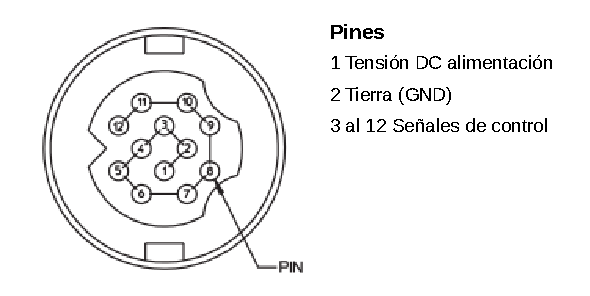
\includegraphics[width=0.6\textwidth]{Imagenes/PinoutConectorViking.pdf}
	\caption{Descripción de pines de un conector Viking}
	\label{Fig:PinoutViking}
\end{figure} 

\begin{figure}[h!]
	\centering
	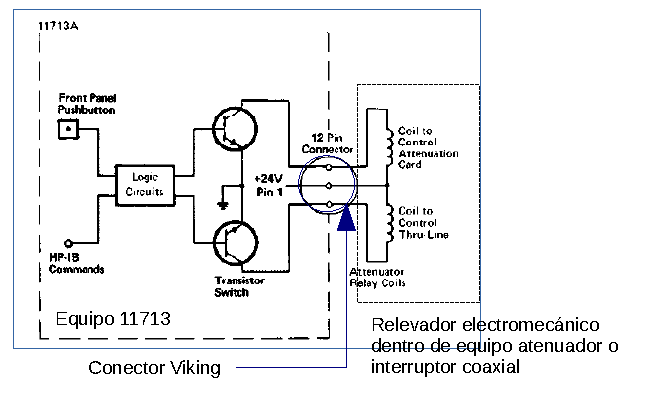
\includegraphics[width=0.8\textwidth]{Imagenes/DiagramaInternoConectorViking.pdf}
	\caption{Diagrama interno generación de señales en conectores Viking}
	\label{Fig:DiagramaInternoConectorViking}
\end{figure}

Los conectores banana ubicados en el panel posterior en los equipos 11713 (figura 8) están destinados al comando de interruptores electromecánicos coaxiales. Están dispuestos en parejas y etiquetados como A y B. En los  modelos 11713A y 11713B existen dos pares de éstos (S0 y S9) y en el modelo 11713C posee cuatro pares con las etiquetas S0 y S9 (Bank1 y Bank2). En la figura 11 se muestra un diagrama del driver interno para estos puertos. Ambos jacks bananas, A y B, generan una señal de tipo binaria y trabajan de forma complementaria, esto significa que cuando un jack presenta la tensión de tierra (0 V) el jack complementario presenta una tensión DC. Cada grupo de conectores S0 y S9 disponen de un jack banana común con un suministro de alimentación DC, para los interruptores que la requieran. Esta tensión de alimentación en los equipos 11713A y 11713B es fija en +24 V DC. En el modelo 11713C esta tensión es puede ser programada por el usuario a un valor fijo de +5, +15 y 25 VDC o ajustada a un valor entre 0 y +24V DC.

\begin{figure}[h!]
	\centering
	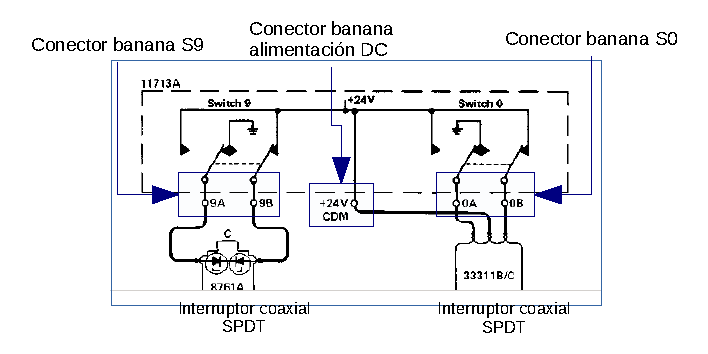
\includegraphics[width=0.8\textwidth]{Imagenes/DiagramaInternoJackBanana.pdf}
	\caption{Diagrama interno generación de señales en jack banana}
	\label{Fig:DiagramaInternoJackBanana}
\end{figure}

En el sistema para medición de ruido de la figura 1, un equipo de la serie 11713 se emplea con un doble propósito, servir como interfaz de usuario y controlador del banco de atenuadores N2002. El estado de cada pareja de pines en un conector Viking en el panel posterior de estos equipos esta relacionado en forma directa con el estado del un botón en el panel frontal. En la tabla 2 se indica esta relación. Los botones en el panel frontal ubicados en la sección etiquetado como Attenuator X controlan el estado de los pines ubicados en el conector Viking del panel posterior etiquetado como ATTEN X. Se cumple una relación idéntica para los botones en la sección etiquetada como Attenuator Y del panel frontal y los conectores Viking etiquetados como ATTEN Y del panel posterior. Por ejemplo los pines 5 y 6 en el conector Viking ATTEN X se corresponde al estado del botón 1 en la sección Attenuator X. De la misma forma, los pines 5 y 6 del conector Viking ATTEN Y responden al estado del botón 5 de la sección Attenuator Y.

\begin{table}[h!]
	\centering
	\begin{tabular}{cc}
		\toprule
		\textbf{Pines} 				&	\textbf{Controlado por botones}			\\
		\textbf{ATTENX y ATTEN Y}	&	\textbf{Attenuator X, Attenuator Y} 	\\
		\midrule
		1	&	Alimentación 	\\
		\midrule
		2	&	Tierra 			\\
		\midrule		
		5	&	\multirow{2}{*}{Botón 1 para ATTEN X Botón 5 para ATTEN Y} \\
		6	&																		\\
		\midrule		
		7	&	\multirow{2}{*}{Botón 2 para ATTEN X Botón 6 para ATTEN Y}	\\
		8	&																		\\
		\midrule		
		9	&	\multirow{2}{*}{Botón 3 para ATTEN X Botón 7 para ATTEN Y}	\\	
		10	&													 					\\
		\midrule		
		11	&	\multirow{2}{*}{Botón 4 para ATTEN X Botón 8 para ATTEN Y}	\\
		12	&																		\\ 
																						 														
		\bottomrule		 
	\end{tabular}
	\caption{Relación de botones panel frontal con los pines en puertos Viking}
	\label{Tab:RelacionBotonesPuertosViking11713}
\end{table}

Los pines en los puertos Viking operan en pareja y de forma complementaria, cuando un pin se encuentra a tierra (GND) su pareja correspondiente se encuentra en alta impedancia. En la tabla 3 se indica la relación que existe  entre el estado de los botones en el panel frontal y el estado de los pines en los conectores Viking. Por ejemplo, cuando el botón 1 del panel Attenuator X se encuentra encendido, en el respectivo conector Viking ATTEN X, el pin 5 se encuentra a tierra (GND) mientras que su pin complementario se encuentra en alta impedancia. Cuando el mismo botón se apaga, los pines 5 y 6 intercambian de estado.

\begin{table}[h!]
	\centering
	\begin{tabular}{ccccc}
		\toprule
		\multicolumn{2}{c}{\bfseries Botones Attenuators} &
		\multirow{2}{*}{\bfseries Estado del botón} & 
		\multicolumn{2}{c}{\bfseries Pines puerto ATTEN} \\
		X & Y &			& Pin & Estado \\
		\midrule
		\multirow{4}{*}{1} & \multirow{4}{*}{5} 
			& \multirow{2}{*}{OFF}    & 5 & GND		\\
			&  &                      & 6 & Hi-Z	\\
			&  & \multirow{2}{*}{ON}  & 5 & Hi-Z	\\
			&  &                      & 6 & GND		\\
		\midrule			
		\multirow{4}{*}{2} & \multirow{4}{*}{6} 
		& \multirow{2}{*}{OFF}    & 7 & GND		\\
		&  &                      & 8 & Hi-Z	\\
		&  & \multirow{2}{*}{ON}  & 7 & Hi-Z	\\
		&  &                      & 8 & GND		\\
		\midrule			
		\multirow{4}{*}{3} & \multirow{4}{*}{7} 
		& \multirow{2}{*}{OFF}    &  9 & GND		\\
		&  &                      & 10 & Hi-Z	\\
		&  & \multirow{2}{*}{ON}  &  9 & Hi-Z	\\
		&  &                      & 10 & GND	\\		
		\midrule			
		\multirow{4}{*}{4} & \multirow{4}{*}{8} 
		& \multirow{2}{*}{OFF}    & 11 & GND		\\
		&  &                      & 12 & Hi-Z	\\
		&  & \multirow{2}{*}{ON}  & 11 & Hi-Z	\\
		&  &                      & 12 & GND	\\				
		\bottomrule
	\end{tabular}
	\caption{Configuracion de botones y su relación con el estado de los pines en los uertos Viking}
	\label{Tab:RelacionBotonesEstodoPinesViking11713}
\end{table}

Los jack banana presentes en el panel posterior, etiquetados como A y B bajo las secciones S9 y S0, también operan por parejas, su estado es complementario y es función del estado presente en los botones del panel frontal, etiquetados como S9 y S0. La tabla 4 resume la relación que existe entre los botones S9 y S0 con los niveles de tensión presentes en los jack banana A y B de las secciones S9 y S0. Por ejemplo, de la tabla 4 se observa que cuando el botón S9 esta encendido (ON), en la sección S9 del panel posterior el estado el jack banana A  se encuentra puesto a tierra (0 V) mientras que el jack banana B presenta una tensión positiva DC (+24 V en el 11713 A). Si ahora el botón S9 se apaga (OFF), los jacks banana A y B de la sección S9 intercambian de estado.

\begin{table}[h!]
	\begin{tabular}{|c|c|c|c|c|}
		\hline
		\multirow{2}{*}{\bfseries Interruptor coaxial} & \multirow{2}{*}{\bfseries Estado botones S9 y S0} & \multicolumn{3}{c}{\bfseries Tensión jack banana panel posterior} \\
		\cline{3-5}
			& 	&	\textbf{Jack}	&	\textbf{A}	&	\textbf{B}  \\
		\hline
		\multirow{2}{*}{S9} & OFF 	& S9 	& +\si{\volt} DC 	& GND \\
		\cline{2-5}
							& ON	& S9	& GND				& +\si{\volt} DC \\
		\hline
		\multirow{2}{*}{S0} & OFF 	& S0 	& +\si{\volt} DC 	& GND \\
		\cline{2-5}
							& ON	& S0	& GND				& +\si{\volt} DC \\
		\hline								
		
	\end{tabular}
	\caption{Relación entre los botones S9 y S0 en el panel frontal y los jacks banana en el panel posterior}
	\label{Tab:RelacionBotonesJackBanana11713}
\end{table}]

En el sistema para medición de figura de ruido, el banco de atenuadores N2002 permite el paso de ciertos intervalos de frecuencia de acuerdo al estado de los botones en el panel frontal de un equipo de la serie 11713.   En la tabla 5 se muestran los rangos de frecuencia de las señales para las cuales el N2002 permite el paso en función del estado de los botones en las secciones Attenuator X y Attenuator Y del panel frontal de un 11713. De esta tabla, cuando los interruptores S9 y S0 están presionados, el N2002 admite el paso de señales cuyas frecuencias se encuentre entre 10 MHz y 3 GHz. Cuando los botones 1 y 5 de las secciones respectivas Attenuator X y  Attenuator Y del panel frontal están presionados, el N2002 admite el paso de señales con frecuencias comprendidas entre 3 GHz y 6 GHz.

\begin{table}[h]
	\centering
	\begin{tabularx}{0.6\textwidth}{|c|c|c|c|c|c|c|c|c|c|c|}
		\hline
		\multirow{3}{*}{\bfseries Rango de frecuencia} &
		\multicolumn{8}{c}{Atenuadores} & 
		\multicolumn{2}{c}{\multirow{2}{*}{Interruptores}} \\	
				& \multicolumn{4}{c}{\bfseries Attenuator X} 
				& \multicolumn{4}{c}{\bfseries Attenuator Y} \\
		\cline{2-11}				
				  						& 1 & 2 & 3 & 4 & 5 & 6 & 7 & 8  & S9 & S0 \\
		\hline
		10 a < 3000 \si{\mega\hertz}    &   &   &   &   &   &   &   &    &  X &  X \\
		3 a 6 \si{\giga\hertz} 			& X &   &   &   & X &   &   &    &    &    \\
		< 6 a 12 \si{\giga\hertz}		&   &   & X &   &   &   & X &    &    &    \\				
		> 12 a 18 \si{\giga\hertz}		&   & X &   &   &   & X &   &    &    &    \\
		> 18 a 26.5 \si{\giga\hertz}	&   &   &   & X &   &   &   & X  &    &    \\	
		
		\hline
		
	\end{tabularx}
	\caption{Relación entre los rangos de frecuencia de paso de banda en el N2002 y la combinación de botones en un equipo 11713}
	\label{Tab:ControlRangoFrecuencia11713}
\end{table}
	
	